\documentclass{article}
\usepackage{graphicx}
\graphicspath{{./figs/}}{}
\usepackage{listings}
\title{
HLS-Assignment 6
}
\begin{document}
\maketitle
\hfill \textbf{Sampath Govardhan} \\
\null \hfill \textbf{FWC22071}\\

\section{Problem Statement}
\begin{lstlisting}
Implement a 16bit shift register in HLS. The module should take 3
inputs: 16bit data value, 16bit shift value, and 1 bit left or right
shift flag. Shift value is the value by which you need to shift (in the
direction denoted by shift flag) the data value and produce the output
(also 16bit). Implement it in the most efficient manner possible.

\end{lstlisting}
\vspace{13cm}

\section{Design Code}
\begin{lstlisting}
#include"hls_stream.h"
#include "ap_int.h"
using namespace std;

typedef ap_uint<16> int16;

void a6(int16 a,int16 b, bool s, int16 &out){   //s=0?left:right;
	  for(int i=1;i<=b;i++){
//#pragma HLS PIPELINE
#pragma HLS LOOP_TRIPCOUNT
		  if (s==0){
		  a=a*2;      //out = a<<b;   //out = a * 2^b //left shift
		  }

                  else{
		  a=a/2;     //out = a>>b;   //out = a / 2^b //right shift
                  }
	  out=a;
          }
}


\end{lstlisting}
\vspace{15cm}


\section{Test Bench Code}
\begin{lstlisting}
#include "hls_stream.h"
#include "ap_int.h"
#include <iostream>
#include <fstream>
using namespace std;

typedef ap_uint<16> int16;

void a6(int16 a,int16 b, bool s, int16 &out);

int main(){
	ap_uint<16> a,b,out,d;
	bool s,f;
	ifstream in("in.dat");
	ofstream res("out.dat");

	for (int i=0;i<6;i++){
	in>>a>>b>>s>>d;
	a6(a, b, s, out);
	res<<a<<"\t"<<b<<"\t"<<s<<"\t"<<d<<"\t";
	if (out==d){
		res<<out<<"\t"<<"Pass"<<endl;;
	}
	else{
		res<<out<<"\t"<<"Fail"<<endl;
		f++;
	}
	}
   if (f==0){
	   cout<<"ALL TEST CASES ARE PASSED!"<<endl;
   }
   else{
	   cout<<"ERROR! ALL TEST CASES ARE NOT PASSED"<<endl;
   }

	return 0;
}

\end{lstlisting}
\vspace{13cm}
\section{C Simulation Output}
\begin{lstlisting}
INFO: [SIM 2] *************** CSIM start ***************
INFO: [SIM 4] CSIM will launch GCC as the compiler.
   Compiling ../../../../a6.cpp in debug mode
   Generating csim.exe
ALL TEST CASES ARE PASSED!
INFO: [SIM 1] CSim done with 0 errors.
INFO: [SIM 3] *************** CSIM finish ***************

\end{lstlisting}
\vspace{3cm}
\section{in.dat file}
\begin{lstlisting}
5 2 0 20
5 2 1 1
10 1 1 5
10 1 0 20
1 7 0 128
1 7 1 0


\end{lstlisting}
\vspace{3cm}
\section{out.dat file}
\begin{lstlisting}
5	2	0	20	20	Pass
5	2	1	1	1	Pass
10	1	1	5	5	Pass
10	1	0	20	20	Pass
1	7	0	128	128	Pass
1	7	1	0	0	Pass


\end{lstlisting}
\vspace{15cm}


\section{HLS Resource Consumption}
\vspace{3cm}
\begin{figure}[h]
    \centering
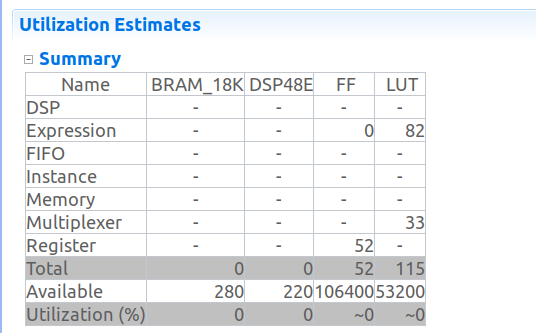
\includegraphics[width=\columnwidth]{1.png}
    \caption{Resource Consumption}
    \label{fig:my_label}
\end{figure}

\vspace{5cm}


\section{HLS Timing Report}
\vspace{1cm}
\begin{figure}[h]
    \centering
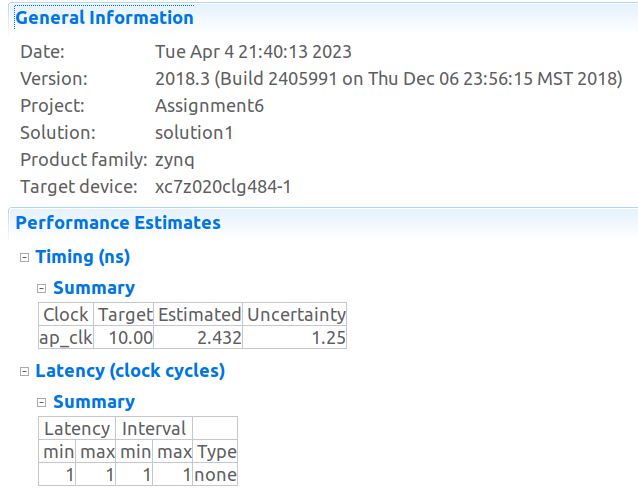
\includegraphics[width=\columnwidth]{figs/2.png}
    \caption{Timing Report}
    \label{fig:my_label}
\end{figure}

\vspace{10cm}


\section{Interfaces Report}
\vspace{1cm}
\begin{figure}[h]
    \centering
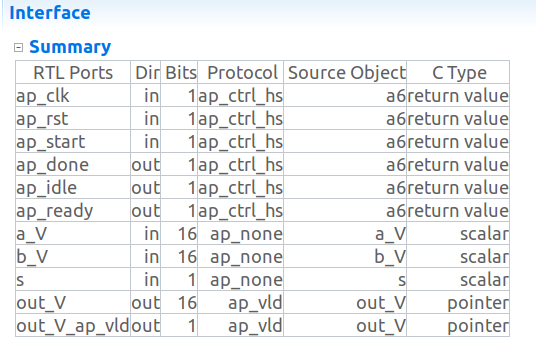
\includegraphics[width=\columnwidth]{figs/3.png}
    \caption{Interface Summmary}
    \label{fig:my_label}
\end{figure}
\vspace{5cm}

\section{C/RTL Cosimulation Output}
\begin{lstlisting}

Starting C/RTL cosimulation ...
/tools/Xilinx/Vivado/2018.3/bin/vivado_hls /home/sam-admin/git/Training/HLS_Assignments/A6/codes/Assignment6/solution1/cosim.tcl
INFO: [HLS 200-10] Running '/tools/Xilinx/Vivado/2018.3/bin/unwrapped/lnx64.o/vivado_hls'
INFO: [HLS 200-10] For user 'sam-admin' on host 'sampaths-lappie' (Linux_x86_64 version 5.19.0-38-generic) on Tue Apr 04 21:40:42 IST 2023
INFO: [HLS 200-10] On os Ubuntu 22.04.2 LTS
INFO: [HLS 200-10] In directory '/home/sam-admin/git/Training/HLS_Assignments/A6/codes'
INFO: [HLS 200-10] Opening project '/home/sam-admin/git/Training/HLS_Assignments/A6/codes/Assignment6'.
INFO: [HLS 200-10] Opening solution '/home/sam-admin/git/Training/HLS_Assignments/A6/codes/Assignment6/solution1'.
INFO: [SYN 201-201] Setting up clock 'default' with a period of 10ns.
INFO: [HLS 200-10] Setting target device to 'xc7z020clg484-1'
INFO: [COSIM 212-47] Using XSIM for RTL simulation.
INFO: [COSIM 212-14] Instrumenting C test bench ...
   Build using "/tools/Xilinx/Vivado/2018.3/tps/lnx64/gcc-6.2.0/bin/g++"
   Compiling a6.cpp_pre.cpp.tb.cpp
   Compiling a6_tb.cpp_pre.cpp.tb.cpp
   Compiling apatb_a6.cpp
   Generating cosim.tv.exe
INFO: [COSIM 212-302] Starting C TB testing ... 
ALL TEST CASES ARE PASSED!
INFO: [COSIM 212-333] Generating C post check test bench ...
INFO: [COSIM 212-12] Generating RTL test bench ...
INFO: [COSIM 212-323] Starting verilog simulation. 
INFO: [COSIM 212-15] Starting XSIM ...
INFO: [XSIM 43-3496] Using init file passed via -initfile option "/tools/Xilinx/Vivado/2018.3/data/xsim/ip/xsim_ip.ini".
Vivado Simulator 2018.3
Copyright 1986-1999, 2001-2018 Xilinx, Inc. All Rights Reserved.
Running: /tools/Xilinx/Vivado/2018.3/bin/unwrapped/lnx64.o/xelab xil_defaultlib.apatb_a6_top glbl -prj a6.prj -L smartconnect_v1_0 -L axi_protocol_checker_v1_1_12 -L axi_protocol_checker_v1_1_13 -L axis_protocol_checker_v1_1_11 -L axis_protocol_checker_v1_1_12 -L xil_defaultlib -L unisims_ver -L xpm --initfile /tools/Xilinx/Vivado/2018.3/data/xsim/ip/xsim_ip.ini --lib ieee_proposed=./ieee_proposed -s a6 
Multi-threading is on. Using 6 slave threads.
WARNING: [XSIM 43-3431] One or more environment variables have been detected which affect the operation of the C compiler. These are typically not set in standard installations and are not tested by Xilinx, however they may be appropriate for your system, so the flow will attempt to continue.  If errors occur, try running xelab with the "-mt off -v 1" switches to see more information from the C compiler. The following environment variables have been detected:
    LIBRARY_PATH
INFO: [VRFC 10-2263] Analyzing SystemVerilog file "/home/sam-admin/git/Training/HLS_Assignments/A6/codes/Assignment6/solution1/sim/verilog/glbl.v" into library work
INFO: [VRFC 10-311] analyzing module glbl
INFO: [VRFC 10-2263] Analyzing SystemVerilog file "/home/sam-admin/git/Training/HLS_Assignments/A6/codes/Assignment6/solution1/sim/verilog/a6.v" into library xil_defaultlib
INFO: [VRFC 10-311] analyzing module a6
INFO: [VRFC 10-2263] Analyzing SystemVerilog file "/home/sam-admin/git/Training/HLS_Assignments/A6/codes/Assignment6/solution1/sim/verilog/a6.autotb.v" into library xil_defaultlib
INFO: [VRFC 10-311] analyzing module apatb_a6_top
Starting static elaboration
Completed static elaboration
Starting simulation data flow analysis
Completed simulation data flow analysis
Time Resolution for simulation is 1ps
Compiling module xil_defaultlib.a6
Compiling module xil_defaultlib.apatb_a6_top
Compiling module work.glbl
Built simulation snapshot a6


****** Webtalk v2018.3 (64-bit)
  **** SW Build 2405991 on Thu Dec  6 23:36:41 MST 2018
  **** IP Build 2404404 on Fri Dec  7 01:43:56 MST 2018
    ** Copyright 1986-2018 Xilinx, Inc. All Rights Reserved.


source /home/sam-admin/git/Training/HLS_Assignments/A6/codes/Assignment6/solution1/sim/verilog/xsim.dir/a6/webtalk/xsim_webtalk.tcl -notrace
INFO: [Common 17-206] Exiting Webtalk at Tue Apr  4 21:41:24 2023...


****** xsim v2018.3 (64-bit)
  **** SW Build 2405991 on Thu Dec  6 23:36:41 MST 2018
  **** IP Build 2404404 on Fri Dec  7 01:43:56 MST 2018
    ** Copyright 1986-2018 Xilinx, Inc. All Rights Reserved.


source xsim.dir/a6/xsim_script.tcl
# xsim {a6} -autoloadwcfg -tclbatch {a6.tcl}
Vivado Simulator 2018.3
Time resolution is 1 ps
source a6.tcl
## run all
////////////////////////////////////////////////////////////////////////////////////
// Inter-Transaction Progress: Completed Transaction / Total Transaction
// Intra-Transaction Progress: Measured Latency / Latency Estimation * 100%
//
// RTL Simulation : "Inter-Transaction Progress" ["Intra-Transaction Progress"] @ "Simulation Time"
////////////////////////////////////////////////////////////////////////////////////
// RTL Simulation : 0 / 6 [0.00%] @ "125000"
// RTL Simulation : 1 / 6 [100.00%] @ "175000"
// RTL Simulation : 2 / 6 [100.00%] @ "215000"
// RTL Simulation : 3 / 6 [100.00%] @ "245000"
// RTL Simulation : 4 / 6 [100.00%] @ "275000"
// RTL Simulation : 5 / 6 [100.00%] @ "365000"
// RTL Simulation : 6 / 6 [100.00%] @ "455000"
////////////////////////////////////////////////////////////////////////////////////
$finish called at time : 495 ns : File "/home/sam-admin/git/Training/HLS_Assignments/A6/codes/Assignment6/solution1/sim/verilog/a6.autotb.v" Line 404
## quit
INFO: [Common 17-206] Exiting xsim at Tue Apr  4 21:41:32 2023...
INFO: [COSIM 212-316] Starting C post checking ...
ALL TEST CASES ARE PASSED!
INFO: [COSIM 212-1000] *** C/RTL co-simulation finished: PASS ***
Finished C/RTL cosimulation.


\end{lstlisting}

\section{C/RTL Cosimulation Report}
\vspace{1cm}
\begin{figure}[h]
    \centering
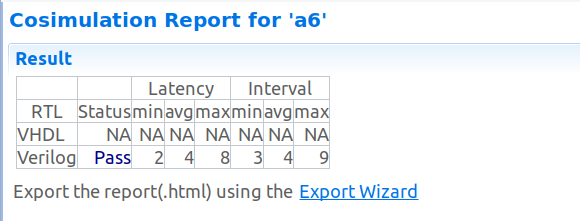
\includegraphics[width=\columnwidth]{figs/4.png}
    \caption{Cosimulation Report}
    \label{fig:my_label}
\end{figure}
\end{document}
